\chapter[Project Planning]{PROJECT PLANNING}

\section{Software Requirements}
	After literature survey and studies, the top tools that were found for our project are as follows:

	\begin{itemize}
		\item \textbf{Machine learning training:} PyTorch, Huggingface Transformers, and Optimum.
		\item \textbf{Machine learning inference:} ONNX Runtime.
		\item \textbf{Web backend:} Express.
		\item \textbf{Web frontend:} HTML, JS, CSS.
		\item \textbf{Database:} Apache Cassandra.
	\end{itemize}

\section{Hardware Requirements}
	In accordance to the software requirements, hardware requirements for our project are as follows:

	\begin{itemize}
		\item \textbf{User devices:} Smartphones, tablets, laptops, and desktop computers.
		\item \textbf{Camera:} Integrated or attachable camera.
		\item \textbf{CPU:} Multi-core 2.5 GHz.
		\item \textbf{GPU:} Minimum 8GB VRAM for training. And any Vulkan-enabled GPU for end-user.
		\item \textbf{Internet connectivity:} Stable internet connection.
	\end{itemize}

\section{Project Scope}
	The scope of the project is as follows:
	
	\begin{itemize}
		\item \textbf{Fashion embedding:} Embed clothing items in higher-dimensional space.
		\item \textbf{Feature extractor:} Train feature extractor to use in segmentation of body parts.
		\item \textbf{AI-based recommender:} Train a personalized recommendation system.
		\item \textbf{Image synthesis virtual try-on:} Develop an image synthesis-powered virtual try-on module.
	\end{itemize}

\section{Project Timeline}
	Probable date of project completion is by the end of the term. A month-by-month distribution and estimation of milestones is as follows:

	\begin{table}[h!]
		\renewcommand{\arraystretch}{1.5}
		\caption{Project Timeline}
		\label{table:timeline}
		\begin{tabularx}{\columnwidth}{
			>{\centering\arraybackslash}p{1.5cm}
			X
		}
			\toprule
				\textbf{Month} & \textbf{Milestones} \\
			\midrule
				1 & Team formation, guide allocation, ideation and topic finalization. \\
				2 & Literature review, feasibility study, scope finalization. \\
				3 & Requirement analysis, high-level architecture design. \\
				4 & Stage-I review. \\
			\addlinespace \hline \addlinespace
				5 & Prototyping, data collection, pipeline setup. \\
				6 & Development and integration. \\
				7 & Testing, optimization, polish. \\
				8 & Stage-II review. \\
			\addlinespace \hline \addlinespace
				Future & Continuous integration and deployment. \\
			\bottomrule
		\end{tabularx}
	\end{table}

    \begin{figure}
        \centering
        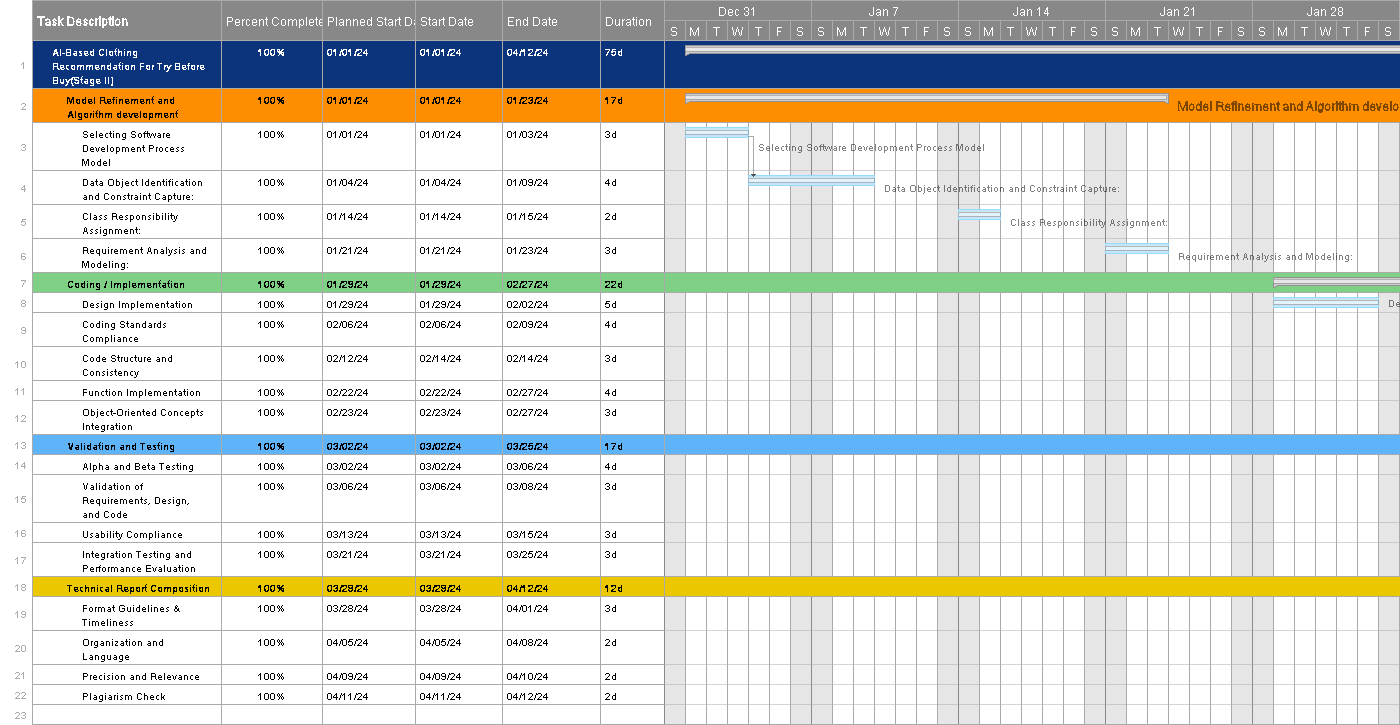
\includegraphics[width=1\textwidth]{components/images/timeline1.png}
        \caption{Project Timeline (Phase 1)}
        \label{fig:recomm}
    \end{figure}
    \begin{figure}
        \centering
        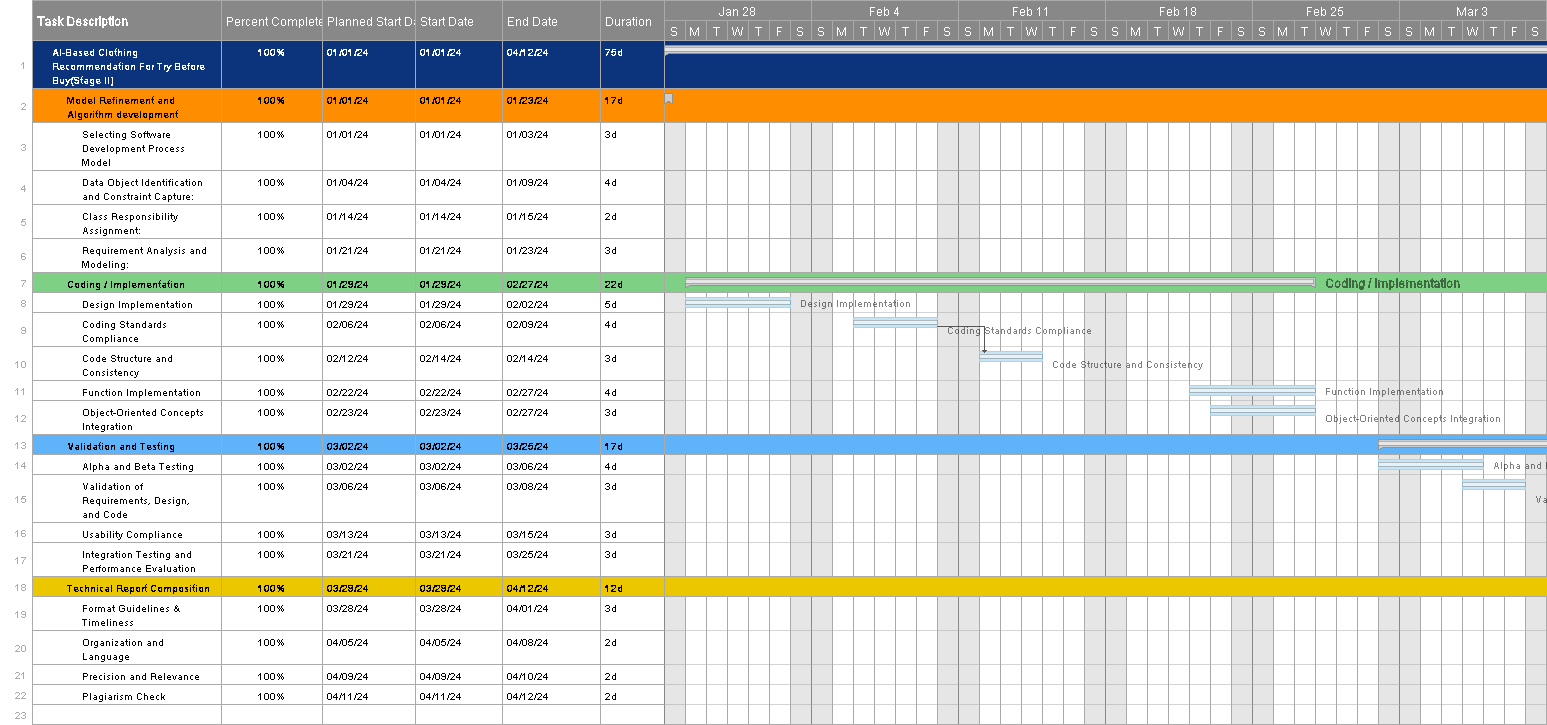
\includegraphics[width=1\textwidth]{components/images/timeline2.png}
        \caption{Project Timeline (Phase 2)}
        \label{fig:recomm}
    \end{figure}
    \begin{figure}
        \centering
        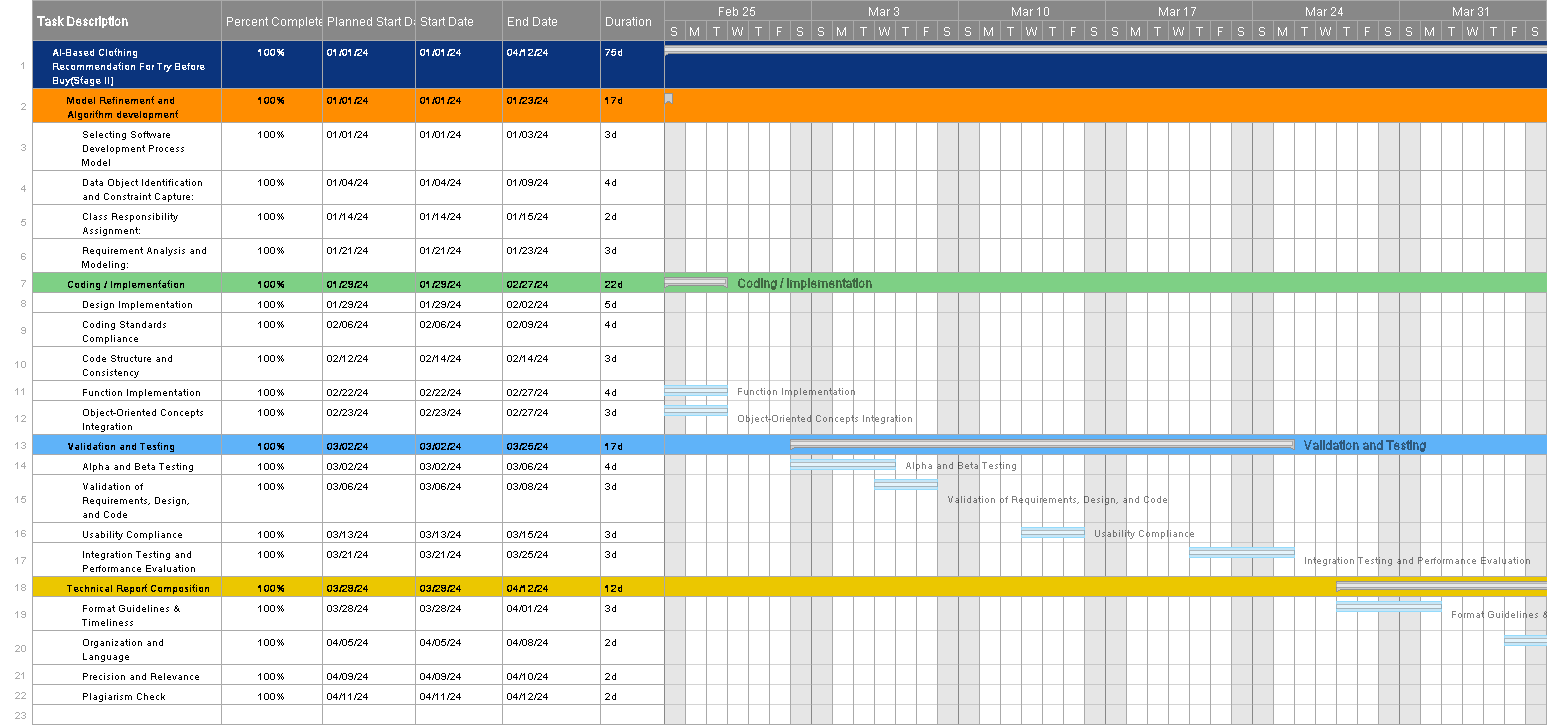
\includegraphics[width=1\textwidth]{components/images/timeline3.png}
        \caption{Project Timeline (Phase 3)}
        \label{fig:recomm}
    \end{figure}
    \begin{figure}
        \centering
        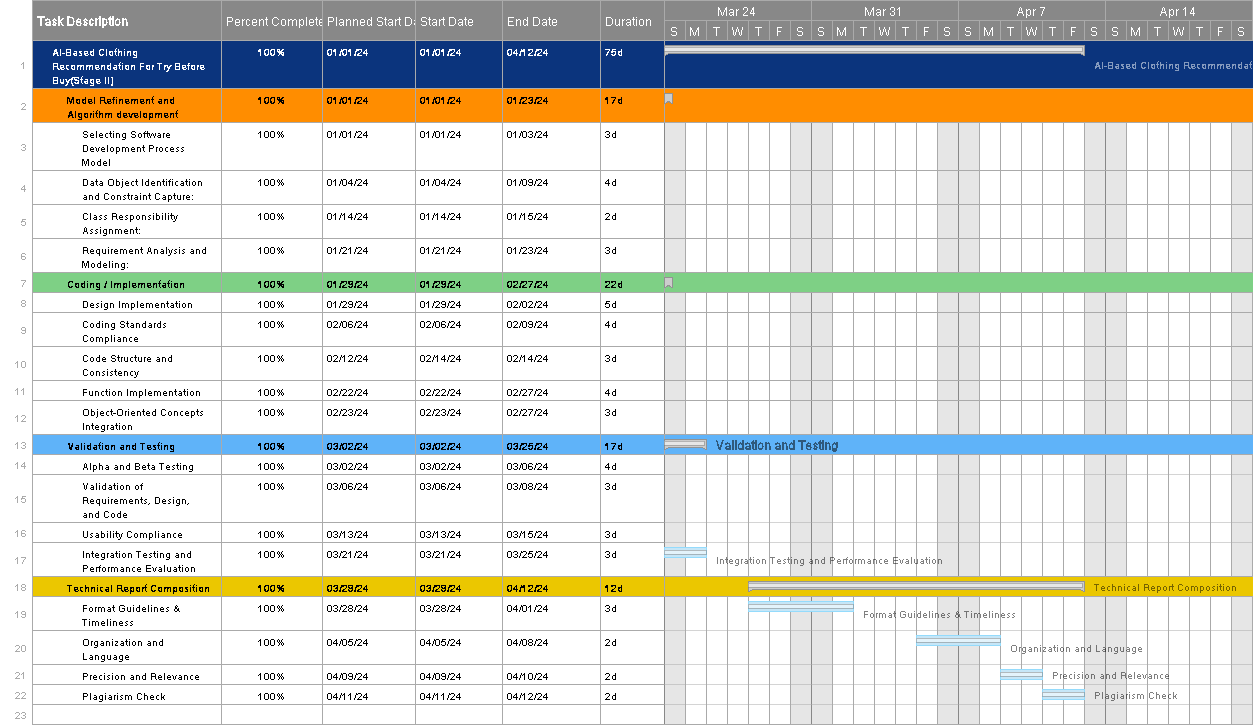
\includegraphics[width=1\textwidth]{components/images/timeline4.png}
        \caption{Project Timeline (Phase 4)}
        \label{fig:recomm}
    \end{figure}